\documentclass[12pt]{article}
\usepackage[paperwidth=15.8in,paperheight=7.0in,margin=0.18in]{geometry}
\usepackage[T1]{fontenc}
\usepackage{lmodern}
\usepackage{amsmath}
\usepackage{xcolor}
\usepackage{tikz}
\usetikzlibrary{arrows.meta,positioning,shapes.geometric}

\definecolor{psidblue}{HTML}{1E3A5F}
\definecolor{psidline}{HTML}{D1D5DB}
\definecolor{psidpanel}{HTML}{F7FAFC}
\definecolor{psidaccent}{HTML}{E8F1FB}
\definecolor{psidgold}{HTML}{A16207}

\pagestyle{empty}
\setlength{\parindent}{0pt}
\setlength{\parskip}{0pt}

\tikzset{
  flowstep/.style={
    rectangle,
    rounded corners=6pt,
    draw=psidblue,
    fill=psidpanel,
    very thick,
    align=center,
    text width=3.6cm,
    minimum height=1cm,
    font=\sffamily\small
  },
  flowwide/.style={flowstep, text width=4.4cm},
  flowresult/.style={flowstep, draw=psidgold!85!black, fill=psidaccent},
  flowarrow/.style={-{Stealth[length=3mm]}, very thick, draw=psidblue}
}

\begin{document}
\thispagestyle{empty}
\centering
\resizebox{0.98\textwidth}{!}{%
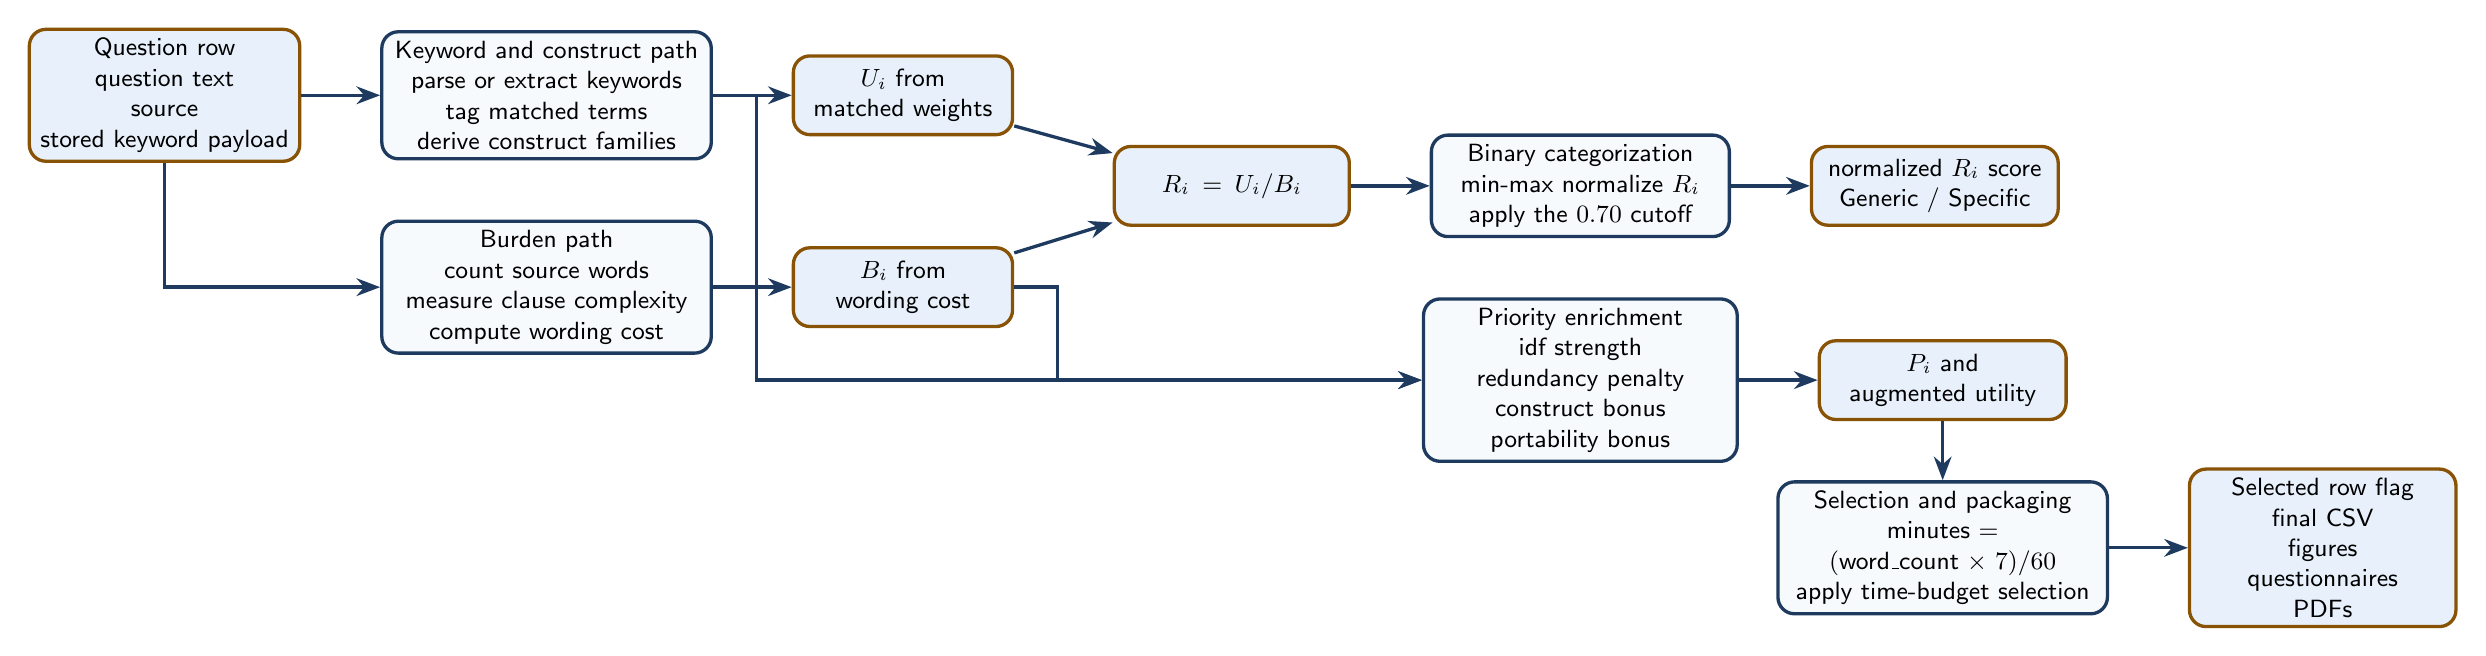
\begin{tikzpicture}[node distance=0.75cm and 1.0cm]
\node[flowresult, text width=3.2cm] (text) {Question row\\question text\\source\\stored keyword payload};
\node[flowstep, right=of text, text width=3.95cm] (keywords) {Keyword and construct path\\parse or extract keywords\\tag matched terms\\derive construct families};
\node[flowstep, below=of keywords, text width=3.95cm] (burden) {Burden path\\count source words\\measure clause complexity\\compute wording cost};
\node[flowresult, right=of keywords, text width=2.55cm] (utility) {$U_i$ from\\matched weights};
\node[flowresult, right=of burden, text width=2.55cm] (burdenv) {$B_i$ from\\wording cost};
\node[flowresult, right=1.25cm of utility, yshift=-1.15cm, text width=2.75cm] (ri) {$R_i = U_i / B_i$};
\node[flowstep, right=of ri, text width=3.55cm] (threshold) {Binary categorization\\min-max normalize $R_i$\\apply the $0.70$ cutoff};
\node[flowresult, right=of threshold, text width=2.9cm] (category) {normalized $R_i$ score\\Generic / Specific};
\node[flowstep, below=of threshold, text width=3.75cm] (augment) {Priority enrichment\\idf strength\\redundancy penalty\\construct bonus\\portability bonus};
\node[flowresult, right=of augment, text width=2.9cm] (pi) {$P_i$ and\\augmented utility};
\node[flowstep, below=of pi, text width=3.95cm] (select) {Selection and packaging\\minutes $= (\text{word\_count} \times 7)/60$\\apply time-budget selection};
\node[flowresult, right=of select, text width=3.15cm] (outputs) {Selected row flag\\final CSV\\figures\\questionnaires\\PDFs};
\draw[flowarrow] (text) -- (keywords);
\draw[flowarrow] (text) |- (burden);
\draw[flowarrow] (keywords) -- (utility);
\draw[flowarrow] (burden) -- (burdenv);
\draw[flowarrow] (utility) -- (ri);
\draw[flowarrow] (burdenv) -- (ri);
\draw[flowarrow] (ri) -- (threshold);
\draw[flowarrow] (threshold) -- (category);
\draw[flowarrow] (keywords.east) -- ++(0.55,0) |- (augment.west);
\draw[flowarrow] (burdenv.east) -- ++(0.55,0) |- (augment.west);
\draw[flowarrow] (augment) -- (pi);
\draw[flowarrow] (pi) -- (select);
\draw[flowarrow] (select) -- (outputs);
\end{tikzpicture}
}
\end{document}